\documentclass{article}

\usepackage{hyperref, tablefootnote, color, graphicx, float}
\graphicspath{{../midterm_presentation/figs/}}
\newcommand{\todo}[1]{\textcolor{red}{\textbf{[#1]}}}

\title{PhotoHunter Design Documentation
}

\author{Connor Greenwell \and Ryan Baltenberger
  \and J.\ David Smith \and Aaron Bradshaw
  \and Scott Workman\footnote{Advisor}}

\begin{document}

\maketitle

\section{Overview}
The PhotoHunter project is a system intended to simplify the creation of
datasets for computer vision research by the process of "gamification". The
system is composed of two mobile applications and a web interface. The web
interface allows researchers to specify a set of images based on their needs.
Based on these specifications, the first mobile application generates a list of
descriptions for photos. Users then capture photos matching these descriptions
and submit them in a scavenger-hunt style game. The second mobile application
uses the submitted photos to quiz users. The players are briefly shown the
images and then asked to label them. Based on the most-commonly provided
answer, the correct label for the image can be determined. The labelled images
are then provided to the researchers that requested the dataset. The system
provides entertainment for users and useful datasets for researchers.

\section{Environment}
The web interface and API for the PhotoHunter Project will be built with Go using PostgreSQL for the database. The backend will run on a DigitalOcean Droplet virtual server. The interface will be tested and fitted to the latest versions of the Mozilla Firefox and Google Chrome web browsers. The mobile applications for the PhotoHunter Project will be built using the Apache Cordova API set. This framework allows smartphone applications to be developed using HTML, CSS, and Javascript. The initial target device will be Android.

\section{Module Descriptions and Data Flow}
The overall data flow between the four main components of the PhotoHunter application follows:
\begin{figure}
\centering
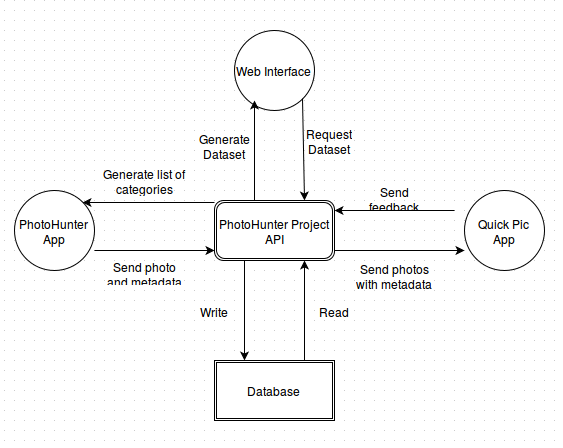
\includegraphics[scale = 0.5]{ss_flowchart}
\end{figure}

\subsection{Researcher Interface}
The researcher interface allows users to request datasets, view the status of any open dataset, and download their dataset.

\paragraph{Create Account}
The create account form allows a new user to register their information in the database. The Go server generates an HTML form requesting the user's name, email address, requested user name, and password. When the user submits the form, the password is encrypted using bCrypt, a Go library, and all information is added to the user table in the database.

\paragraph{Log in to Account}
The login form allows a user to log in to their account. Once a user inputs their user name and password and submits, the Go server selects the user name from the user SQL table, checks the provided password against the correct one, and provides the user with an error message if the account can not be found. If the log in is successful, a new session is created associated with the logged in user.

\paragraph{Update Account}
The account page allows users to update their information. The user may complete an HTML form requesting a new password or providing a new email address. The user's information is then updated in the database.

\paragraph{Request Dataset}
The request dataset functionality allows a user to provide information about a dataset they desire. When a user requests a new dataset, an HTML form is provided allowing the user to specify their needs. The form requires the user to describe the following about the dataset:
\begin{itemize}
\item The subject material of the dataset
\item The time of day that the photos should be taken
\item The location that the photos should be taken
\item The minimum number of photos needed for the dataset
\end{itemize}
If one of these properties is irrelevant to the user, then they may specify that on the form as well. After the dataset is described, the user may submit it to the database.

\paragraph{View Dataset Status}
The researcher interface also allows the user to view the status of their datasets. When this page is viewed, the Go server provides the total count of the photos that currently exist for the dataset.

\paragraph{Download Dataset}
When a dataset has reached the minimum number of photos requested by the user, they may download the dataset from the server. The server gets all images from the dataset and generates a single file containing the metadata for each one. Then each images is compressed and the download is sent to the user.

\begin{figure}[H]
\caption{Researcher Interface Mockup}
\centering
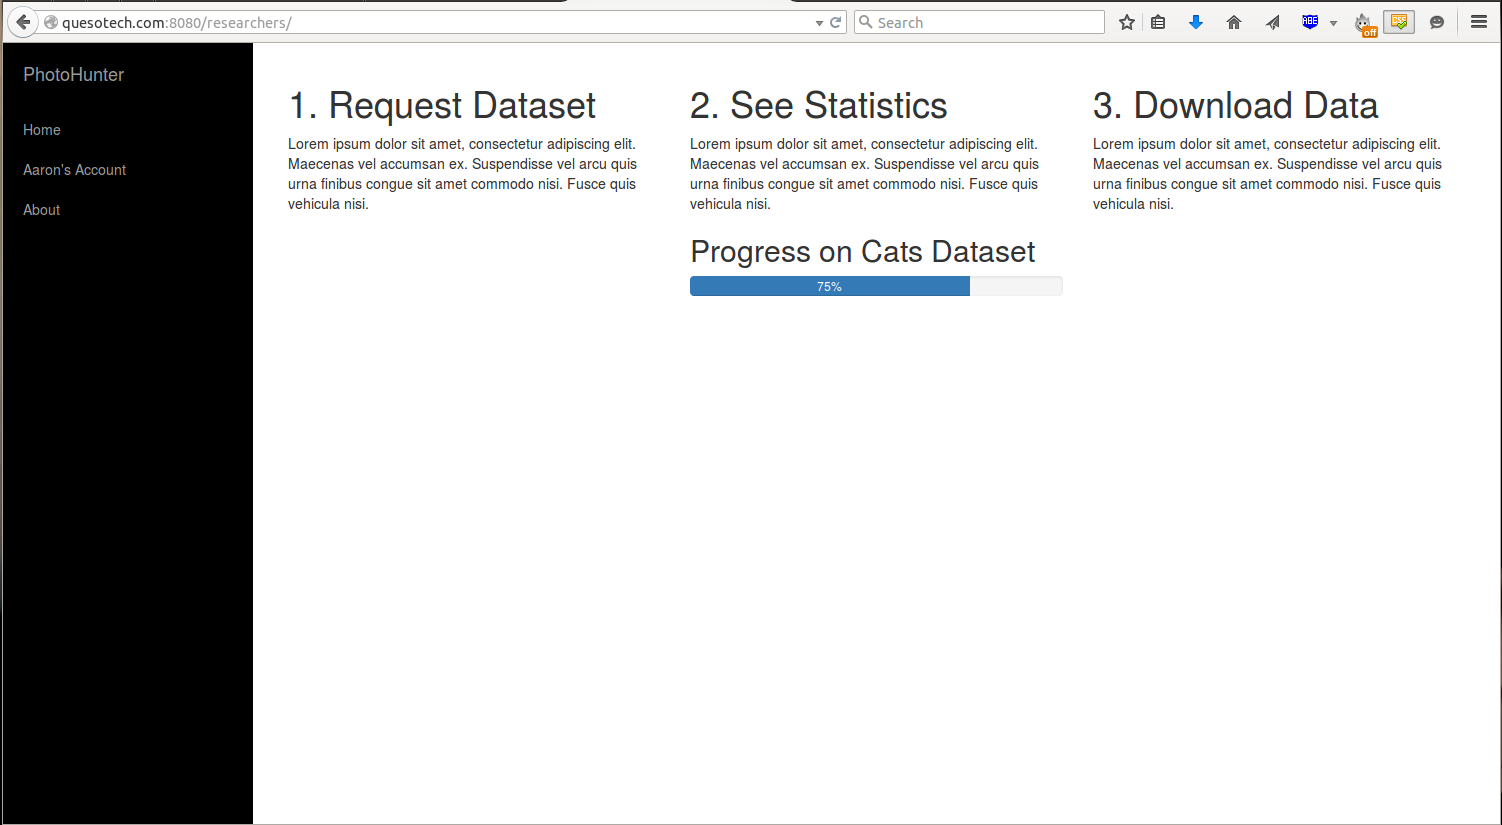
\includegraphics[width=\textwidth,height=\textheight,keepaspectratio]{researchers}
\end{figure}

\subsection{PhotoHunter}
The PhotoHunter application allows users to compete against one another to capture photos in a scavenger hunt.

\paragraph{Create Account/Logging In}
The PhotoHunter application will use a Facebook API to allow users to create accounts and log in using their Facebook accounts.

\paragraph{Provide Lists}
When a user is logged in, the application gets their location data. This data is sent to the PhotoHunter API, which then provides a list of subjects for user to photograph.

\paragraph{Select Topic and Photograph}
The user may choose a topic from the list of available ones. Their smart phone's camera is then opened. After the user takes a photo and confirms it, the application uploads the photo the database. The user's points are then updated in the database.

\paragraph{Leaderboards}
The user may view their ranking against other PhotoHunter users based on their score. This view pulls down the point data from the database, and allows user to narrow their search by location.

\begin{figure}[H]
\caption{PhotoHunter Scavenger List Mockup}
\centering
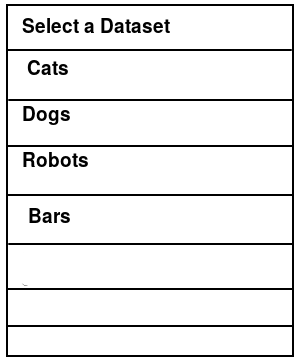
\includegraphics[width =\textwidth, height=\textheight, keepaspectratio]{ss_photohunter_dataset}
\end{figure}

\begin{figure}[H]
\caption{PhotoHunter Upload Mockup}
\centering
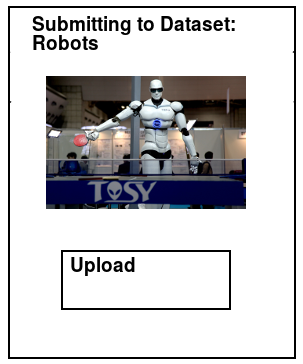
\includegraphics[width =\textwidth, height=\textheight, keepaspectratio]{ss_photohunter_upload}
\end{figure}

\subsection{Quick Pic}
The Quick Pic application allows users to compete against one another by quickly identifying the subjects of images.

\paragraph{Create Account/Logging In}
The Quick Pic application will use a Facebook API to allow users to create accounts and log in using their Facebook accounts.

\paragraph{Quiz}
When a user has logged in, they may begin a quiz. The quiz takes images from the database that were submitted by the PhotoHunter application, and generates four choices. One of these choices is the expected subject, based on the dataset that the image was submitted to in PhotoHunter. The application shows the user the image for a brief second, then asks the user to choose the correct label. The user's answer is then submitted to the database. The user then receives a number of points based on the answers given by other users.

\paragraph{Leaderboards}
The user may view their ranking against other Quick Pic users based on their score. This view pulls down the point data from the database, and allows user to narrow their search by location.

\begin{figure}[H]
\caption{Quick Pic Image Mockup}
\centering
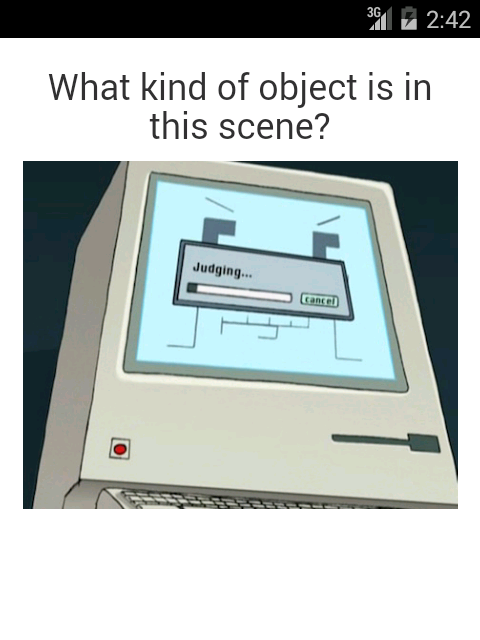
\includegraphics[width =\textwidth, height=\textheight, keepaspectratio]{ss_quickpic_image}
\end{figure}

\begin{figure}[H]
\caption{Quick Pic Options Mockup}
\centering
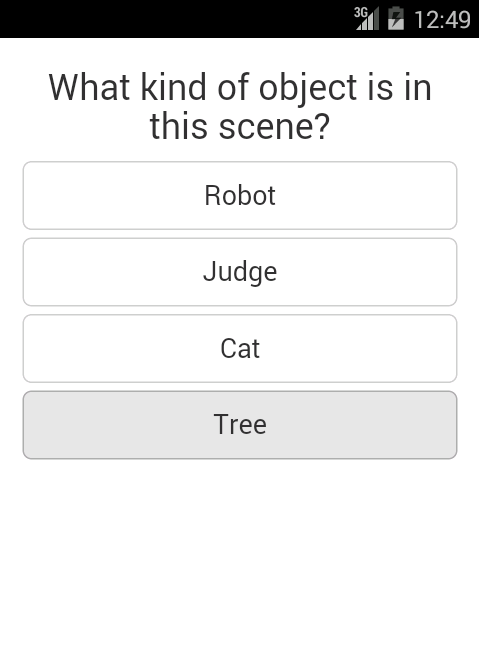
\includegraphics[width =\textwidth, height=\textheight, keepaspectratio]{ss_quickpic_options}
\end{figure}

\subsection{API}

\paragraph{Create Dataset from Request}

Members of Research Teams (RTs) will provide Requests, which describe
the kind of data the RTs are looking for.  The internals of the API will
generate PhotoHunter and QuickPic jobs to collect data for the
Requests.

\paragraph{Generate Scavenger Lists for PhotoHunter}

Scavenger Lists are the jobs generated for PhotoHunter.  For a given
Request, one scavenger list entry for each requirement presented in
the request. For example, if the RT requests the following dataset:

\begin{itemize}
  \item Cats or Dogs
  \item Between 1pm and 8pm EST
\end{itemize}

Then the API will generate the following scavenger list entries:

\begin{itemize}
  \item Dogs Between 1pm and 8pm EST
  \item Cats Between 1pm and 8pm EST
\end{itemize}

The Request is expected to already have the data laid out in such a
manner that constructing this list is trivial (essentially the cartesian
product of elements of lists).

These Scavenger Lists will be made available to the PhotoHunter application
with some constraints.  The constraints are to be designed to avoid presenting
users with entries that are infeasible for them to complete.  The initial set
of constraints is:

\begin{itemize}
\item Do not show users entries for which they are spatially ineligible (ie RT
  requests images from New York City, but user is in New Hampshire)
\item Do not show users entries for which the non-repeating time requirement
  has already passed (example: RT requests images for the month of February,
  2015, but it is now March, 2015)
\end{itemize}

More constraints may be added based on further brainstorming, development and
testing with input from the customer.

\paragraph{Add Photo to Dataset}

When a Scavenger List entry is completed by a user of the PhotoHunter
application, a Photo is submitted to the API.  The API will store the Photo in
a database, along with both the dataset it was captured for and the entry that
the user claimed it matched.  This information with be available to the
requesting RT.

\paragraph{Get Photo and Labels for Quick Pic}

The QuickPic application will request Photo and Label data from the API at a
rate of 1 Photo at a time.  Each response will include the Photo and 4 Labels.
The set of Labels will include:

\begin{itemize}
  \item The Label claimed by the user who submitted the photo via PhotoHunter
  \item The most popular Label according to QuickPic votes
\end{itemize}

The remaining Labels will be randomly chosen.  If the two required Labels are
the same, then there may be 3 random Labels chosen.

\paragraph{Calculate Points for Both Applications}

Points will be calculated in the following manner:

\begin{itemize}
  \item A base amount (say, 10) is always given simply for completing a task.
  \item Further points may be awarded based on confidence in the choice's
    accuracy.  Accuracy will be determined by comparing to the histogram of
    choices made by other users.  The number of additional points awarded will
    be $90 \times \text{Confidence}$, where Confidence is on the range of
    $[0, 1]$.

  \item Points will be back-propagated to the PhotoHunter application at a rate
    of 1 PhotoHunter point per 10 QuickPic points.  This lowered rate was
    chosen because for each Photo, 1 PhotoHunter user may receive points but
    arbitrarily many QuickPic users may receive points.
\end{itemize}

\textbf{Note: The values of points and rates are subject to change based on
  testing and input from the customer.  These are not necessarily the final
  values.}

\paragraph{Analyse Quick Pic Label Choices}

Label choices from QuickPic will be analyzed using as-of-yet undetermined
statistical methods to determine what the probably True Label is and the
confidence on the Claimed Label.  Information about the choices will be made
available to the Research Teams receiving the images and labels.

The output from this method is important for the \textit{Calculate Points for
  Both Applications} stage.

\paragraph{Compile Dataset}

The Dataset will be compiled based on images received from PhotoHunter and
Labels received from QuickPic.  Anonymized statistical information about images
and labels will be made available to the research team(s) receiving the
dataset(s).

Datasets will be transmitted as compressed archive files (ex: zip, tar.gz) with
labels being stored in csv files.

\section{Use Cases}
\subsection{Researcher Interface}
When visiting the researcher interface, a user may do one of the following:
\begin{itemize}
\item Log In: A user can log in to their account using their credentials. They will then be taken to their dashboard.
\item Create Account: A new user may create an account by signing up.
\end{itemize}

After logging in, a user may visit one of the following pages on the dashboard:
\begin{itemize}
\item Datasets: This page is where the user may do any of the following:
\begin{itemize}
\item Request Dataset: A user may complete an HTML form specifying a dataset that meets their needs. The user may then submit the dataset definition to the database.
\item View Datasets: A user may view the status of their datasets. As new images are submitted, verified, and added to the dataset, the updated number may be viewed by the researcher.
\item Download Dataset: After a dataset is complete, a user may download their dataset.
\end{itemize}
\item Account: This page allows users to update account information, including their email address or password.

\end{itemize}
\subsection{PhotoHunter}

\begin{itemize}
\item Log In: A user can log in to their account using their credentials. They will then be taken to their dashboard.
\item Create Account: A new user may create an account by signing up.
\end{itemize}

After logging in, a user may visit one of the following views:

\begin{itemize}
\item Scavenger List: A list of Scavenger List Entries which have been
  requested by Research Teams. Choosing an entry will launch the native Camera
  application, allowing users to capture and submit a picture.
\item Leaderboard: A view presenting an overview of the top users relative to
  the logged in user for the PhotoHunter application.  Various metrics may be
  presented, such as ``Most Points (All Time)'', ``Most Points (Past Month)'',
  ``Most Submissions (All Time)'', ``Most Points Per Submission (All Time)''.

\item Account: A view allowing the user to update account information.
\end{itemize}

\subsection{Quick Pic}

\begin{itemize}
\item Log In: A user can log in to their account using their credentials. They will then be taken to their dashboard.
\item Create Account: A new user may create an account by signing up.
\end{itemize}

\begin{itemize}
\item Label Images: A user will be presented with an image to label.  The
  amount of time they are given to view the image may depend on their overall
  score.  They will then be asked to choose a label.  Upon choosing a label,
  they will be presented with some information about their accuracy and asked
  to label another image.
\item Leaderboard: A view presenting an overview of the top users relative to
  the logged in user for the PhotoHunter application.  Various metrics may be
  presented, such as ``Most Points (All Time)'', ``Most Points (Past Month)'',
  ``Most Submissions (All Time)'', ``Most Points Per Submission (All Time)''.

\item Account: A view allowing the user to update account information.
\end{itemize}
\section{Design Considerations}
Initially, the mobile applications for the PhotoHunter Project were to be developed for both iOS and Android. However, due to the limited time available and scope of the project, the team decided to develop the applications just for Android. 

\section{Sizing Estimate}
The researcher interface will be handled by a server written in Go. The Go language has several packages to support server development. Hence, the estimated size of the server itself is less than 1000 lines of code. We will use the Bootstrap framework for the front end of the researcher interface, greatly reducing the number of lines of HTML and CSS we need to to write. The API for the application will also be written in Go. As the API does the majority of the work, we estimate it to be ~2000 lines of code. The API will also use SQL to interact with the database. Due to the size of the database and the number of entities, an estimated 1000 lines of SQL will be needed to communicate with the database.

The mobile applications will each be built with Cordova. The Cordova framework generates boilerplate code automatically. This reduces the number of lines needed to complete a working application. However, we still estimate a total of 2000 lines each for the two mobile applications.

\section{References}
Following are a list of technologies we intend to use:
\begin{itemize}
\item \href{http://cordova.apache.org/}{Cordova}
\item \href{https://golang.org/}{Google's Go Programming Language}
\item \href{http://www.postgresql.org/}{PostgreSQL}
\item \href{http://getbootstrap.com/}{Bootstrap Framework}
\end{itemize}

\end{document}
